%%%%%%%%%%%%%%%%%%%%%%%%%%%%%%%%%%%%%%%%%%%%%%%%%%%
%% P3: Phenomenology of Particle Physics                         
%%
%% Author:  André Rubbia                   		 
%%
%% Figure 15.2 Illustration of the Coulomb potential (dashed curve) and Yukawa potentials (lines).
%%
%% This work is licensed under the Creative Commons Attribution 4.0 International License. 
%% To view a copy of this license, visit http://creativecommons.org/licenses/by/4.0/ or 
%% send a letter to Creative Commons, PO Box 1866, Mountain View, CA 94042, USA.
%%
%%%%%%%%%%%%%%%%%%%%%%%%%%%%%%%%%%%%%%%%%%%%%%%%%%%

\documentclass[a4paper,10pt]{article}

\usepackage[T1]{fontenc}
\usepackage[utf8]{inputenc}
\usepackage{lmodern}
\usepackage[labelfont=bf]{caption}
\usepackage{upgreek}

\usepackage{tikz}
\usepackage{pgfplots}
\pgfplotsset{compat=1.17}
\usepgfplotslibrary{ternary}
\usepgfplotslibrary{fillbetween}
\usepgfplotslibrary{external}

\usepackage{braket}

\def\d{\mathrm{d}}

\pgfkeys{/pgf/number format/.cd,1000 sep={}}

\begin{document}

%%%%%%%%%%%%%%%%% FIGURE %%%%%%%%%%%%%%%%%%%%%%%%%%%%%%%%%%
\begin{figure}[htb]
\begin{center}
\pgfplotsset{every axis/.append
    style={
    width=0.9*\textwidth,
    height=0.7*\textwidth,
    line width=1pt,
    tick style={line width=0.8pt}}}
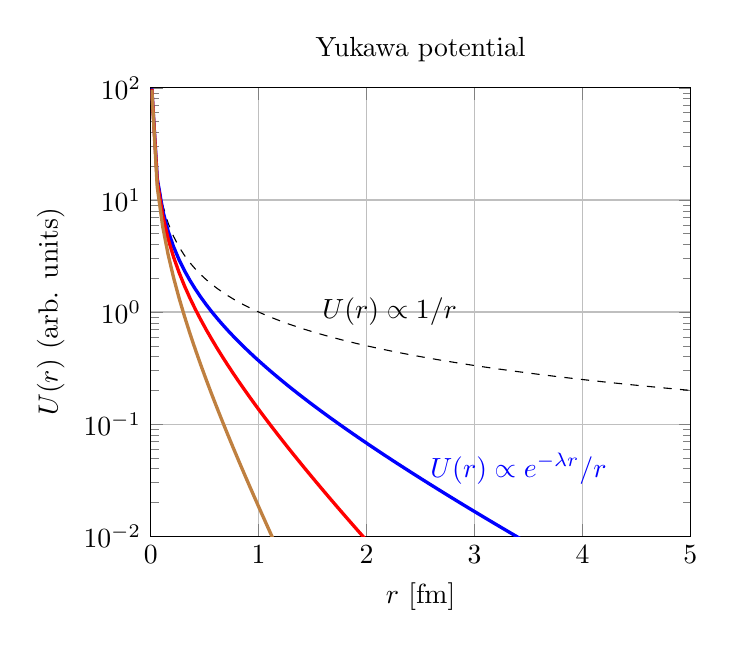
\begin{tikzpicture}[scale=1.]
    \begin{semilogyaxis}[
        title=Yukawa potential,
        xlabel={$r$ [fm]},
        ylabel={$U(r)$ (arb. units)},
        xmin=0, xmax=5,
        ymin = 1e-2, ymax=1e2,
        minor y tick num=1,
        grid = major    ]
        \addplot [black,dashed,domain=0.01:5, samples=100] {1/x};
        %% lambda=1
        \addplot [blue,very thick,domain=0.01:5, samples=100] {exp(-x)/x};
        %% lambda=2
        \addplot [red,very thick,domain=0.01:5, samples=100] {exp(-2*x)/x};
        %% lambda=4
        \addplot [brown,very thick,domain=0.01:5, samples=100] {exp(-4*x)/x};
	 \node[right,black] at (axis cs:1.5,1) {$U(r)\propto 1/r$};
	 \node[right,blue] at (axis cs:2.5,0.04) {$U(r)\propto e^{-\lambda r}/r$};
  \end{semilogyaxis}
\end{tikzpicture}%

\caption{Illustration of the Coulomb potential (dashed curve) and Yukawa potentials (lines)
with the arbitrarily chosen values $\lambda=1$, $2$, and $4$~fm$^{-1}$. The larger the $\lambda$, the
shorter the corresponding range.}
\end{center}
\end{figure}
%%%%%%%%%%%%%%%%% END FIGURE %%%%%%%%%%%%%%%%%%%%%%%%%%%%%%
%

\end{document}
